\documentclass[11pt]{article}
%\usepackage[14pt]{extsizes} % для того чтобы задать нестандартный 14-ый размер шрифта
%\usepackage[utf8]{inputenc}
\usepackage{mathtext}
\usepackage[english, russian]{babel}
\usepackage{amsmath}
\usepackage{amsfonts}
\usepackage{float}
\usepackage[margin=0.8in]{geometry}
\usepackage{multirow}
\usepackage{graphicx}
\usepackage[utf8x]{inputenc} % указать кодировку русского текста
\usepackage{fancyhdr}
\usepackage{indentfirst} % отступ в первой строке абзаца
\usepackage{wrapfig}
\usepackage{placeins}
\usepackage{wrapfig}
\usepackage{caption}
\usepackage{amssymb}
\usepackage{mathtools}
\usepackage[thinc]{esdiff}
\usepackage{cmap}
\usepackage[table,xcdraw]{xcolor}

\usepackage{float}
\restylefloat{table}

\pagestyle{fancy}
\begin{document}
\begin{titlepage}
\begin{center}
%\vspace*{1cm}
\large{\small ФЕДЕРАЛЬНОЕ ГОСУДАРСТВЕННОЕ АВТОНОМНОЕ ОБРАЗОВАТЕЛЬНОЕ\\ УЧРЕЖДЕНИЕ ВЫСШЕГО ОБРАЗОВАНИЯ\\ МОСКОВСКИЙ ФИЗИКО-ТЕХНИЧЕСКИЙ ИНСТИТУТ\\ (НАЦИОНАЛЬНЫЙ ИССЛЕДОВАТЕЛЬСКИЙ УНИВЕРСИТЕТ)\\ ФИЗТЕХ-ШКОЛА РАДИОТЕХНИКИ И КОМПЬЮТЕРНЫХ ТЕХНОЛОГИЙ}
\vfill
\line(1,0){430}\\[1mm]
\huge{Лабораторная работа 4.7.2}\\
\huge\textbf{Эффект Поккельса}\\
\line(1,0){430}\\[1mm]
\vfill
\begin{flushright}
\normalsize{Устюжанина Мария}\\
\normalsize{\textbf{Группа Б01-107}}\\
\end{flushright}
\end{center}
\end{titlepage}
\fancyhead[L] {Работа 4.7.2}

\par \textbf{Цель работы:} исследовать интерференцию рассеянного света, прошедшего кристалл; наблюдать изменение характера поляризации
света при наложении на кристалл электрического поля.

\par \textbf{В работе используются:} гелий-неоновый лазер, поляризатор, кристалл ниобата лития, матовая пластина, экран, источник высоковольтного переменного и постоянного напряжения, фотодиод, осцилограф, линейка.


\section{Теоретическое введение}
  
Эффект Поккельса -- изменение показателя преломления света в кристалле под действием электрического поля.\\
Рассмотрим кристалл ниобата лития $\text{LiNbO}_3$ с цетрольноосевой симметрией вдоль оси $Z$. Для световой волны с $\mathbf{E}$ перпендикулярно $Z$ показатель преломления будет $n_o$, а для волны с $\mathbf{E}$ вдоль $Z$ -- $n_e$. В случае, когда луч света идёт под углом $\theta$ к оси, есть два значение показателя преломления $n_1$ и $n_2$: $n_1 = n_o$ для волны с $\mathbf{E}$ перпендикулярным плоскости $(\mathbf{k},\mathbf{Z})$ (обыкновенная волна) и $n_2$ для волны с $\mathbf{E}$ в этой плоскости (необыкновенная волна). В последнем случае
\begin{equation}
\dfrac{1}{n_2^2}=\dfrac{\cos^2 \theta}{n_0^2}+\dfrac{\sin^2 \theta}{n_e^2}.
\end{equation}

\begin{wrapfigure}{r}{0.5\textwidth}
\begin{center}
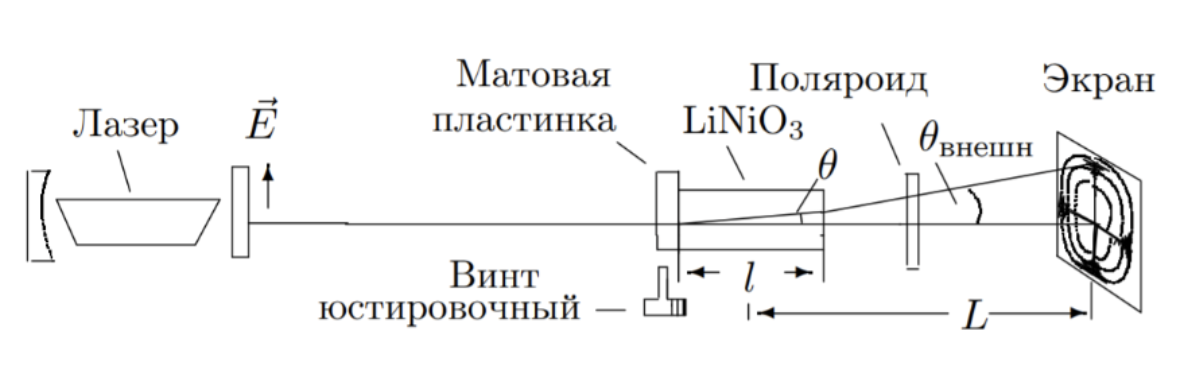
\includegraphics[width = 0.5\textwidth]{1.png}
\end{center}
\vspace{-20pt}
\caption{Схема для наблюдения интерфереционной картины.}
\end{wrapfigure}

Если перед кристаллом, помещённым между поляроидами, расположить линзу или матовую пластинку, то на экране за поляроидом мы увидим тёмные концентрические окружности -- рещультат интерфернции обыкновенной и необыкновенной волн. При повороте выходного поляроида на $90^\circ$ картина меняется с позитива на негатив (на месте светлых пятен тёмные и наоборот). В случаи, когда разрешённое направление анализатора перпендикулярно поляризации лазерного излучения, радиус тёмного кольца с номером $m$ равен
\begin{equation}
r_m^2 = \dfrac{\lambda}{l} \dfrac{(n_oL)^2}{n_0 - n_e}m,
\end{equation}

\begin{wrapfigure}{r}{0.45\textwidth}
\begin{center}
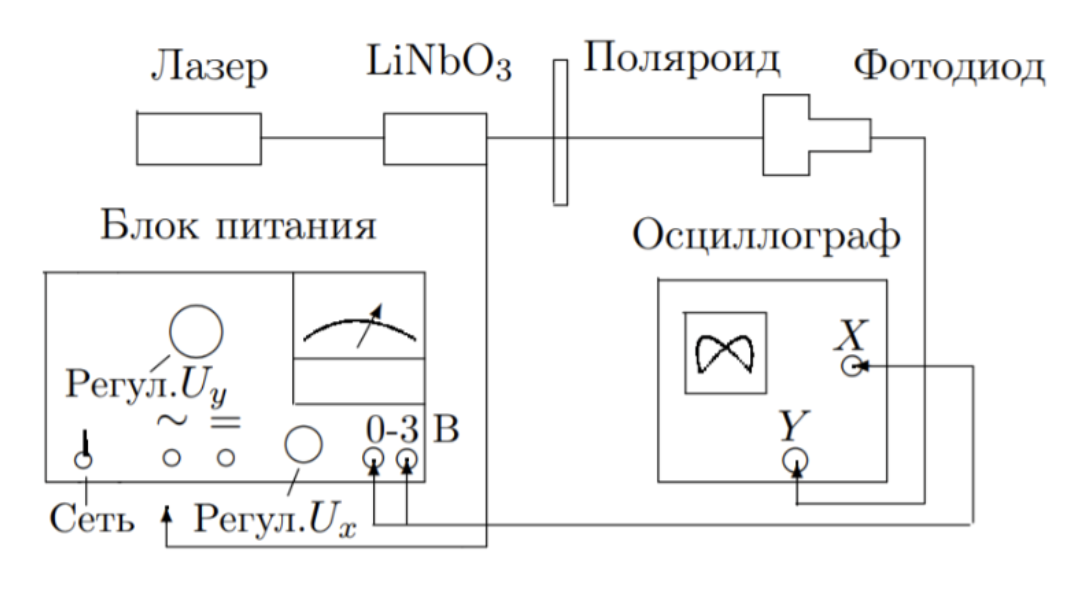
\includegraphics[width = 0.45\textwidth]{2.png}
\end{center}
\vspace{-20pt}
\caption{Схема установки.}
\end{wrapfigure}

где $L$ -- расстояние от центра кристалла до экрана, $l$ -- длина кристалла.\\
Теперь поместим кристалл в постоянное электрическое поле $E_{\text{эл}}$, направленное вдоль оси $X$, перпендикулярной $Z$. Показатель преломления для луча, распространяющего вдоль $Z$, всегда $n_o$. В плоскости $(X,Y)$ возникают два главных направления под углами $45^\circ$ к $X$ и $Y$ с показателями преломления $n_0 - \Delta n$ и $n_o + \Delta n$ (быстрая и медленная ось), причём $\Delta n = A E_{\text{эл}}$. Для поляризованного вертикально света и анализатора, пропускающего горизонтальную поляризацию, на выходе интенсивность на выходе будет иметь вид
\begin{equation}
I_{\text{вых}} = I_0 \sin^2 \left(\dfrac{\pi}{2} \dfrac{U}{U_{\lambda/2}} \right),
\end{equation}
где $U_{\lambda/2} = \frac{\lambda}{4A}\frac{d}{l}$ -- \textit{полуволновое напряжение}, $d$ -- поперечный размер кристалла.  При напряжении $U = E_{\text{эл}}d$ равном полуволновому сдвиг фаз между двумя волнами равен $\pi$, а интенсивность света на выходе максимальна. 


На Рис. 2 представлена схема всей установки (оптическая часть изорбажена на Рис. 1). Свет лазера, проходя через сквозь пластину, рассеивается и падает на двоякопреломляющий кристалл. На экране за поляроидом видна интерференционная картина. Убрав рассеивающую пластину и подавая на кристалл постоянное напряжение, можно величиной напряжения влиять на поляризацию луча, вышедшего из кристалла. Заменив экран фотодиодом и подав на кристалл переменное напряжение, можно исследовать поляризацию с помощью осциллографа.
\newpage


\section{Ход работы:}


\subsection*{Определение разности показателей преломления}

Выполним юстировку системы, получим интерфереционную картину. 

Измерим радиусы $r(m)$ тёмных колец при расстоянии $L =84 \pm 1 \text{ см}$ от середины кристалла до экрана. Результаты занесем в Таблицу 1. На Рис 3 построим график $r^2 = f(m)$.

\begin{table}[h]
\caption{Радиусы тёмных колец.}
\centering
\begin{tabular}{|c|c|c|c|c|c|c|}
\hline
$m$     & 1   & 2   & 3   & 4   & 5   & 6   \\ \hline
$r_m$, см & 2.9 & 4.3 & 5.3 & 6.1 & 6.7 & 7.2  \\ \hline
\end{tabular}
\end{table}[]


\begin{wrapfigure}{r}{0.5\textwidth}
\begin{center}
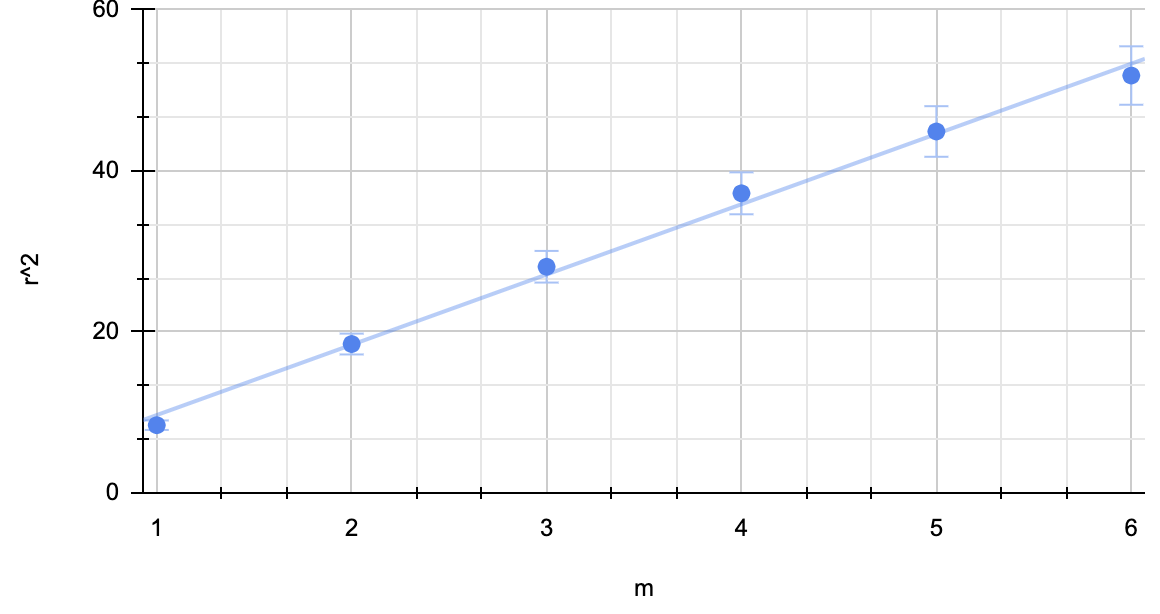
\includegraphics[width = 0.5\textwidth]{gr1.png}
\end{center}
\vspace{-20pt}
\caption{$r^2=f(m)$}
\end{wrapfigure}

Получим $k =  8,6 \pm 0.1 \text{см}^2$. 

Отсюда для значений $n_0 = 2.29$, $\lambda = 0.63 \text{ мкм}$, $l = 26 \text{ мм}$ получаем из формулы (2)
\[
\boxed{n_0 - n_e = 0.1 \pm 0.01}
\]



\subsection*{Определение полуволнового напряжения ниобата лития}
 Убедимся ещё раз, что направление лазерного луча совпадает с направлением на центр интерференционной картины и уберём матовую пластинку. Подключим разъём блока питания на постоянно напряжение, установим регулятор напряжения на минимум и включим блок питания в сеть.

Увеличивая напряжение на кристале определим полуволновое напряжение по максимальной яркости пятна на
экране:
\begin{equation} \label{eq:U0.5}
  U_{\lambda/2} = 435\;В
\end{equation}
И по положению следующего минимума - волновое напряжение
\[ U_{\lambda} = 2 U_{\lambda/2} = 960\; В\]

Проделаем всё то же самое для параллельной поляризации лазера и анализатора:
\[ U_{\lambda/2} = 900\;В\]
\[ U_{\lambda} = 2 U_{\lambda/2} = 1440\;В\]

Вращая анализатор и наблюдая за яркостью пятна на экране, убеждаемся, что поляризация круговая.\\

Дальнейшие измерения проводим при помощи осциллографа. Установим вместо экрана фотодиод и поставим на переменное напряжение. С трёхвольтового
выхода БП подадим сигнал на  \(X\)-канал осциллографа. Таким образом, отклонение луча осциллографа по
оси \(X\) будет пропорционально напряжению \(U\) на кристалле, а по оси \(Y\) - интенсивности прошедшего
через анализатор сигнала \(I_{out}\)

Постепенно повышая напряжение на кристалле, будем наблюдать на экране фигуры Лиссажу, соответсвующие
зависимости \(I_{out}\) для скрещенных поляризаций лазера и анализатора. объ1мся от фигуры Лиссажу
симметричности.

\begin{figure}[H]
  \centering
  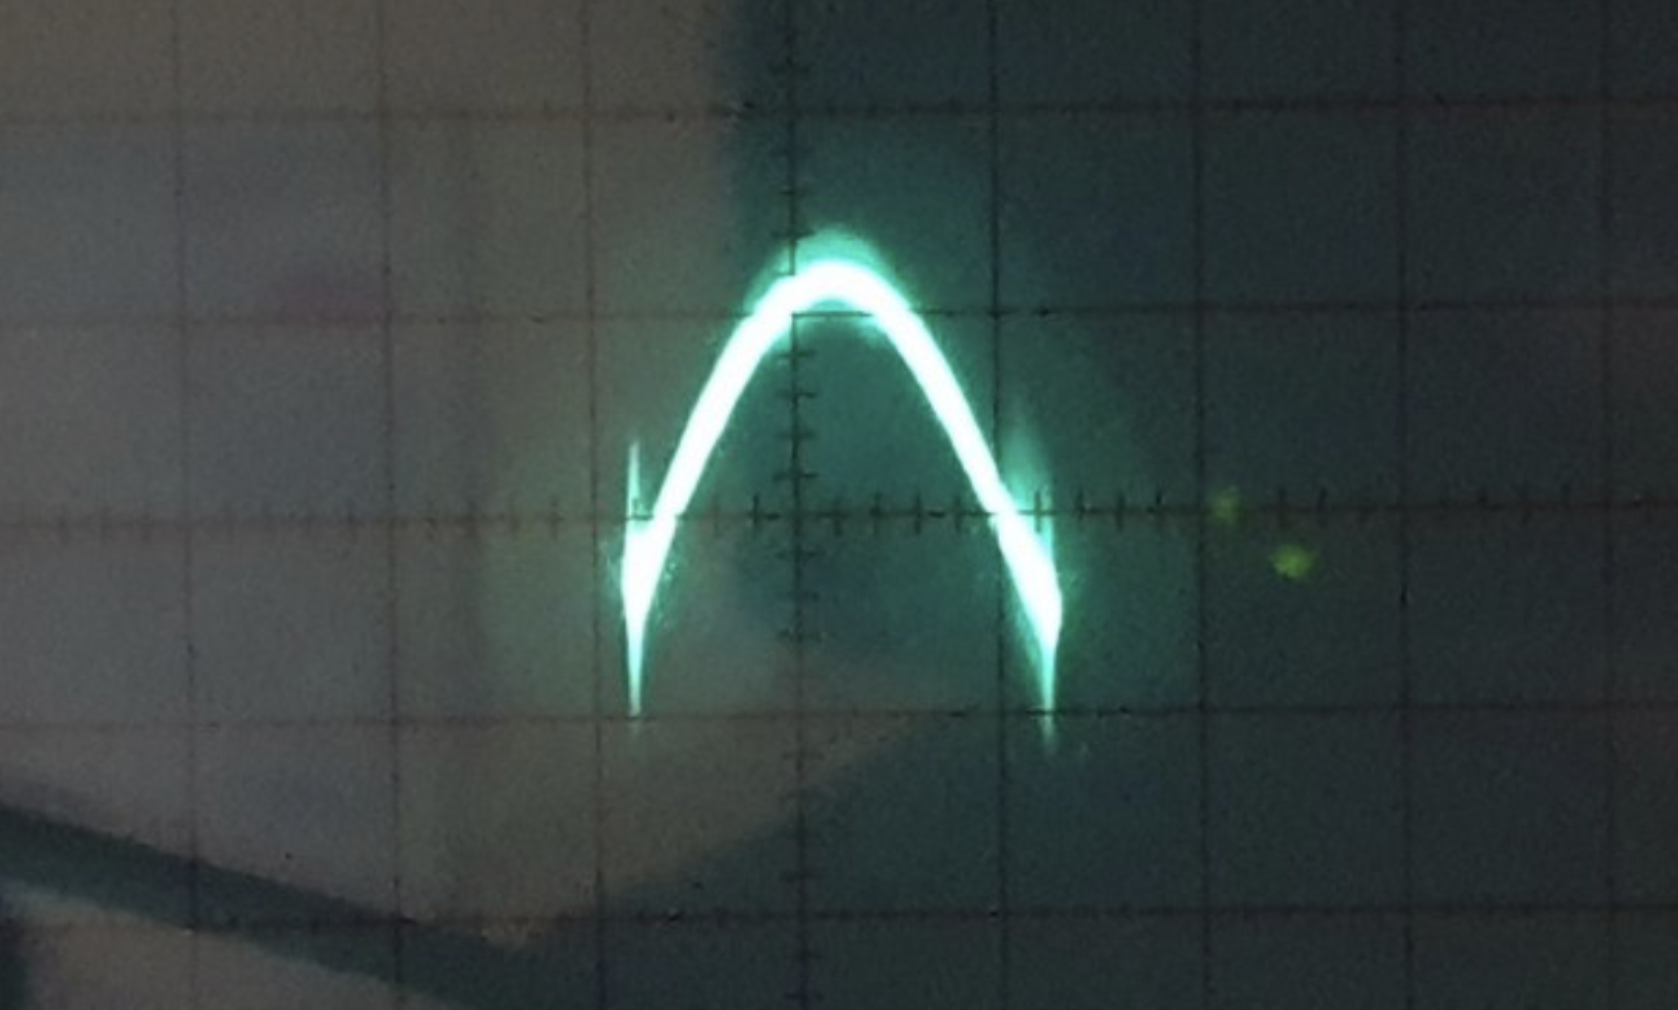
\includegraphics[width=\textwidth]{L1.png}\label{fig:L}
  \caption{Фигура Лиссажу}
\end{figure}

Наблюдая за фигурой Лиссажу, определим (по вольтметру на источнике питания) полуволновое напряжение 
\(U_{\lambda/2}\) как \(\Delta U\), соответствующее переходу от макимума к минимуму на осциллограмме.

\[ U_{\lambda/2} = \Delta U = 480 В\]

Это значение довольно точно совпадает со значением \(U_{\lambda/2}\) для поперечной поляризации, полученным ранее.



\subsection*{Фигуры Лиссажу для различных напряжений}

\begin{figure}[H]
  \centering
  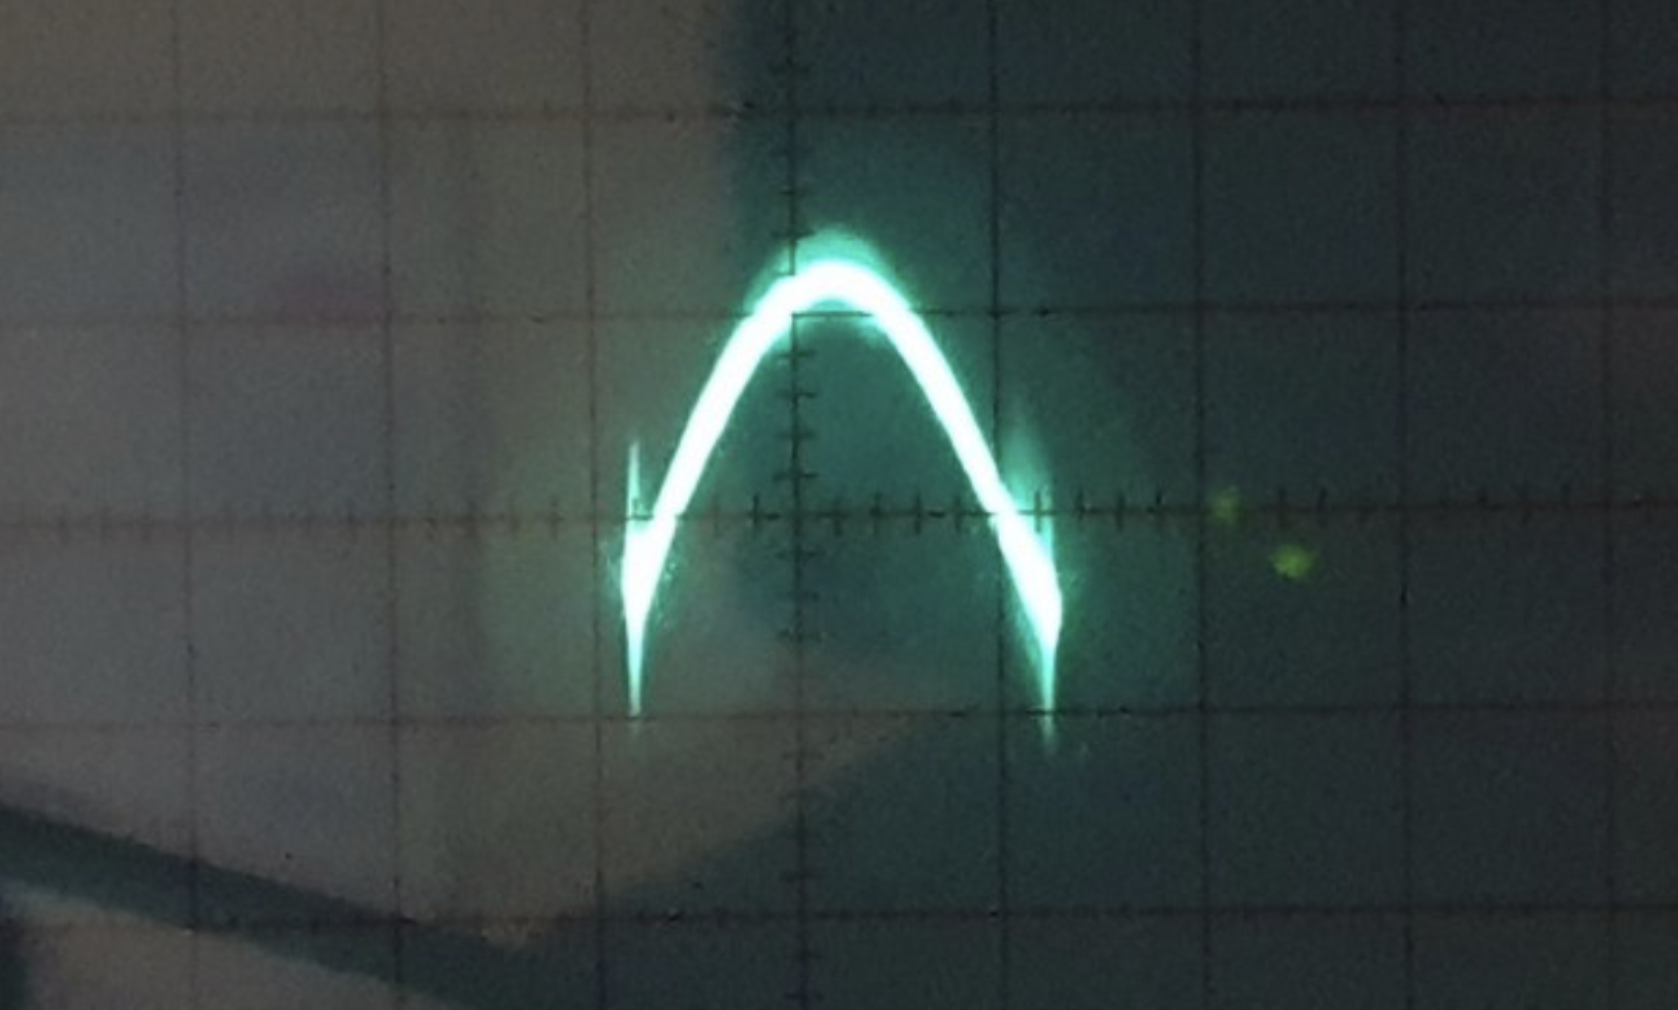
\includegraphics[width=\textwidth]{L1.png}\label{fig:L1}
  \caption{Фигура Лиссажу при \(U = U_{\lambda/2}\)}
\end{figure}

\begin{figure}[H]
  \centering
  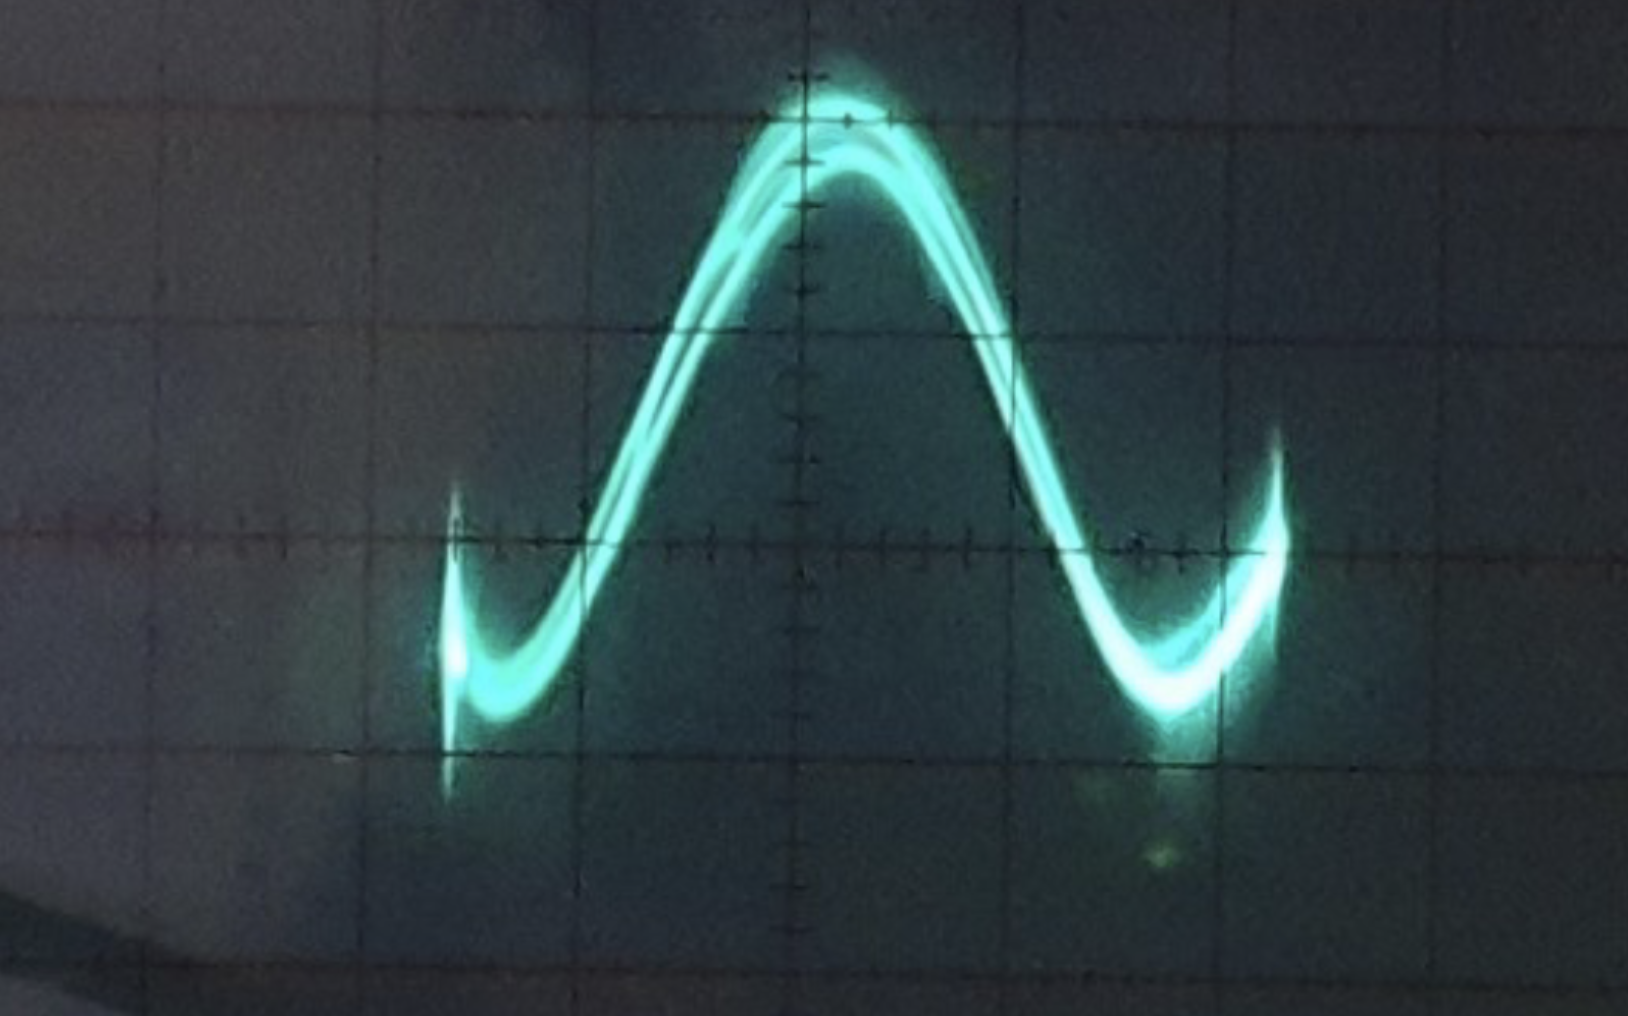
\includegraphics[width=\textwidth]{L2.png}\label{fig:L2}
  \caption{Фигура Лиссажу при \(U = U_{\lambda}\)}
\end{figure}

\begin{figure}[H]
  \centering
  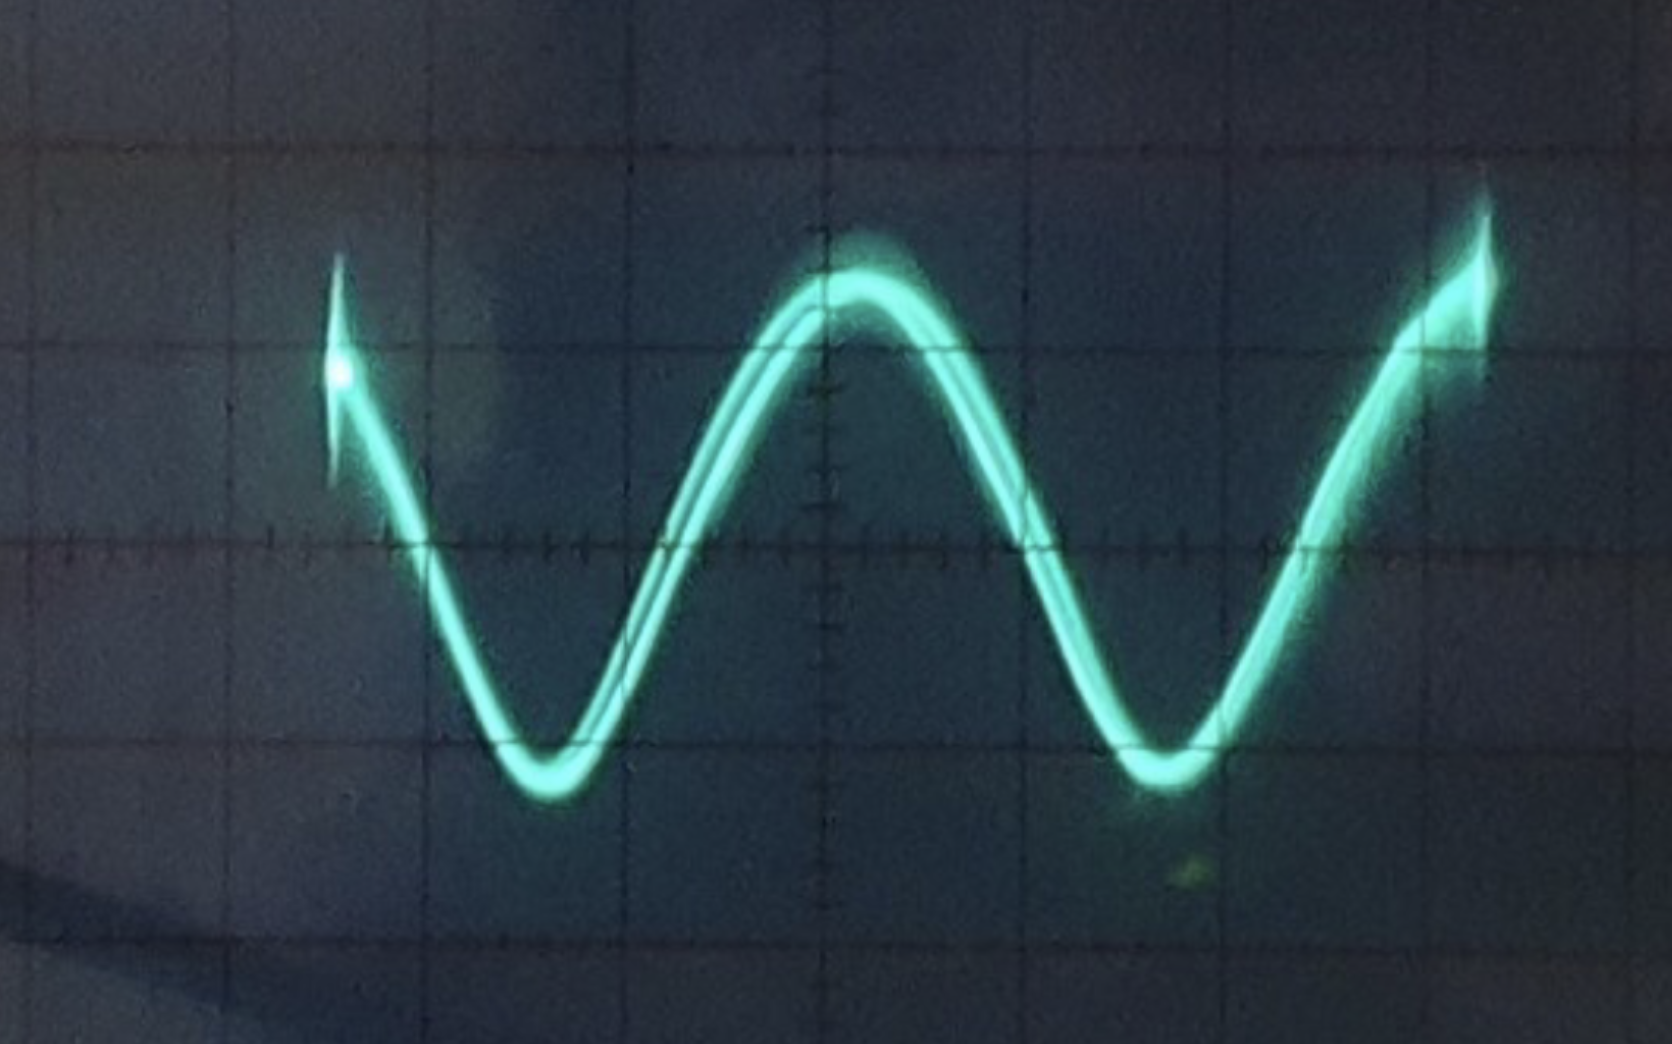
\includegraphics[width=\textwidth]{L3.png}\label{fig:L3}
  \caption{Фигура Лиссажу при \(U = U_{3\lambda/2}\)}
\end{figure}


\section*{Обсуждение результатов и выводы}
\begin{itemize}

\item Было проведено измерение радиусов тёмных колец $r(m)$ на расстоянии $L = 84 \pm 1 $ см от середины кристалла до экрана. Результаты приведены в Таблице 1. Из зависимости $r^2$ от порядкового номера кольца (График 1) аппроксимацией получили угловой коэффициент $k = 8.6 \pm 0.1 \text{ см}^2$. Отсюда для указанных на установке значений $n_0 = 2.29$, $\lambda = 0.63 \text{ мкм}$, $l = 26 \text{ мм}$ для двулучепреломления ниобата лития получили
\[
\boxed{n_0 - n_e = 0.1 \pm 0.01}
\]  
Табличное значение для двулучепреломления ниобата лития: $n_0 - n_e = 0.09$. Видим, что в пределах погрешности оно совпадает с полученным.

\item Было измерено полуполновое напряжение кристалла на длине волны $\lambda = 0.63 \text{мкм}$ при постоянном и переменном напряжениях. Первое определяем из условия максимума интенсивности, второе -- при помощи осциллографа по разности напряжений при максимуме и минимуме у фигуры Лиссажу. Получили 
\[
\boxed{U_{\lambda / 2}^{\text{AC}} = 435 \pm 15 \text{B}},
\boxed{U_{\lambda / 2}^{\text{DC}} = 480 \pm 15 \text{B}}
\]
Видим, что значения достаточно похожи.

\item Подав на кристалл четвертьволновое напряжение, вращая анализатор убедились в том, что поляризация на выходе из кристалла круговая.

\end{itemize}

Основоной вклад в ошибку в ходе выполнения работы могла внести неточность при определении диаметра колец на экране и выходного напряжения при помощи источника питания.

\end{document}